\section{Multiple Imputation}
\begin{frame}{Plan For This Presentation}
  \begin{figure}[h!]
  \centering
    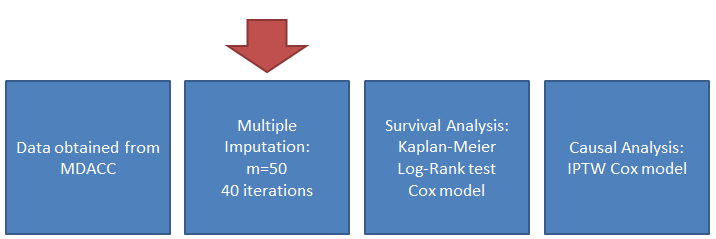
\includegraphics[width=0.9\textwidth]{mi_flow}
\label{fig:mi_flow}
\end{figure} 
\end{frame}

\subsection{Missing Data}
\begin{frame}{Missing data and Historical Approaches}
 \begin{itemize}
 \item Missing data happens when we intend to collect a piece of data but don't actually get it
 \item Historical approaches
 \begin{itemize}
  \item Complete Case (CC) analysis: Throw away any record that is not complete
  % list of downsides
 \item Available Case (AC) analysis: Use records so long as they are complete for the specific analysis in question
 %bad things here
 \item Single Imputation (SI): Fill in the missing value, deduct degrees of freedom to account for it
 \end{itemize}
 \end{itemize}
 
 \note{This can occur because when correlations are computed using different cases,
 the resulting patterns can be ones that are impossible to produce with complete data.}
\end{frame}

\begin{comment}
 
\begin{frame}{Imputation}
\begin{block}{Definition}
The English verb ``to impute'' comes from the Latin imputo, which means
to reckon, attribute, make account of, charge, ascribe. \cite{VanBuuren2012}
\end{block}
\begin{itemize}
 \item In the 1930's, Allan, Wishart, and Yates laid framework for missing data
 \begin{itemize}
  \item Idea: Fill in the missing value, deduct degrees of freedom to account for it
  \item Issue: Dogmatic, and variance can't be estimated correctly
 \end{itemize}

\end{itemize}
\end{frame}

\end{comment}

\subsection{MI Theory}
\begin{frame}{Multiple Imputation}
Throughout the 70's and 80's Donald Rubin worked to improve on single imputation
\begin{itemize}
 \item Instead of imputing one value, lets impute it $m\geq 2$ times
 \item Draw the values from the missing data's posterior distribution given the observed
 data and the process that generated the missing data
\end{itemize}
This idea is called Multiple Imputation (MI) and was formalized in 1987 \cite{Rubin1987}. It is the gold standard method
for missing data currently.

\note{MI are repitions drawn to simulate a Bayesian posterior distribution
of the missing values under a model}

\end{frame}


\begin{frame}{How does MI work?}
 \begin{figure}[h!]
  \centering
    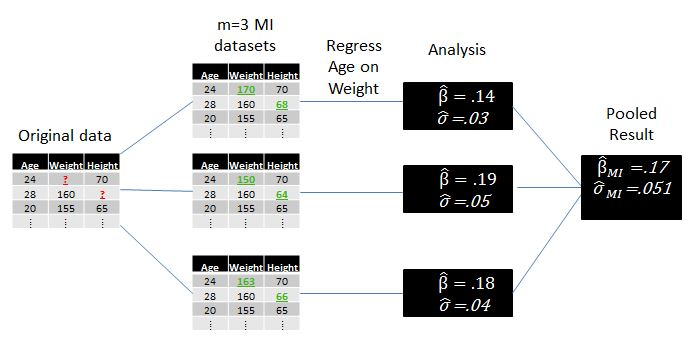
\includegraphics[width=0.8\textwidth]{mi_example_full.jpg}
  \caption{Visualization of MI data}
\label{fig:miexample}
\medskip
\small
Missingness is displayed by \textcolor{red}{?'s} and the imputed data is shown  as \textcolor{teal}{\#'s}.
We then regress age on weight, get the results from the individual datasets, and then pool them together.
\end{figure}
\note{We will go in to much more detail later in presentation}
\end{frame}

\begin{frame}{MI Theory}
 \begin{itemize}
  %\item Assume that the full data comes from $p(Y,X,R|\theta)$
  %\begin{itemize}
  % \item Y are the covariates with missingness
   %\item X is the fully observed covariates
   %\item R is the response missingness indicator
   %\item $\theta$ parameterizes this model
  %\end{itemize}
  \item Missing data model: $p(R|Y_{obs},Y_{mis},\psi)$
  \begin{itemize}
     \item R is the response missingness indicator
   \item $Y_{obs},Y_{mis}$ are observed and missings of Y (the set of covariates with missingness)
   \item $\psi$ parameterizes the missing data model
  \end{itemize}

 \end{itemize}

\end{frame}


\begin{frame}{Missing data Mechanisms}
%notation here?
\begin{itemize}

\item MCAR: Missing completely at random:  $$P(R=0|Y_{obs},Y_{mis},\psi)=P(R=0|\psi)$$
\begin{itemize}
\item The missingness in the data is not at all related to any of the data that we do or don't have
\end{itemize}
\item MAR: Missing at random: $$p(R=0|Y_{obs},Y_{mis},\psi)= p(R=0|Y_{obs},\psi)$$
\begin{itemize}
 \item The missingness we have is related to something in the data 
\end{itemize}
\item MNAR: Missing not at random: $$p(R=0|Y_{obs},Y_{mis},\psi)$$ does not simplify
\begin{itemize}
 \item  and the missingness depends on data that we have as well as have not collected
\end{itemize}
\end{itemize}
\note{
 If a lab technician slips and drops 5 vials of blood, the missingness caused by this would be MCAR
 If we collect the gender of the subject and we know that males tend to not give blood, we can attribute the missingness to the gender. In general, MAR models are ignorable.
 For example if a full moon causes the blood testing machine to break more often, but we don't have the moon phase as a variable.
}
\end{frame}

\begin{frame}{Missing data Example}

 \begin{figure}[h!]
  \centering
    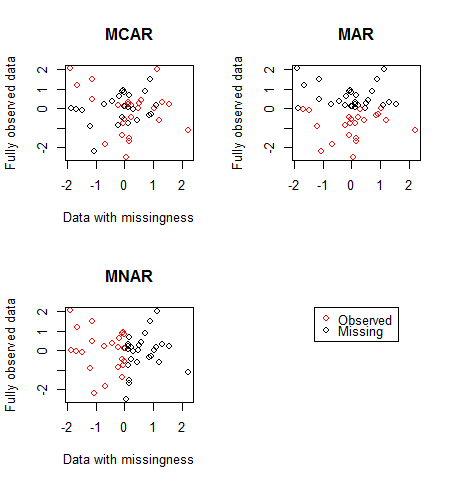
\includegraphics[width=0.63\textwidth]{md_mechanism}
  \caption{Visualization of MI data}
\label{fig:miviz}
\medskip
\small
Missingness is displayed by \textcolor{red}{?'s} and the imputed data is shown  as \textcolor{teal}{\#'s}.
We then regress age on weight, get the results from the individual datasets, and then pool them together.
\end{figure}
 
\end{frame}

\begin{frame}{Full Conditional Specification (FCS)}
 \begin{itemize}
  \item Assume MAR missing data mechanism %although MNAR with more 
  \item Missing data is imputed iteratively on a variable by variable basis
  \item Drawing from $p(Y,X,R|\theta)$ through the full conditionals $p(Y_j|X,Y_{-j},R,\theta_j)$
  \begin{itemize}
   \item X: Fully observed data
   \item $Y_{-j}$ is the missing components without column j
   \item $\theta$ parameterizes full data model
  \end{itemize}

  %\item Requires no distributional assumptions
  %\item Specify univariate models for each missing variable conditional on other variables
  \item Generalization of univariate imputation
  \item Idea: Specify k one dimensional models to impute on the missing data columns
 \end{itemize}

\end{frame}

%I'm going to want to type this up as an algorithm
\begin{frame}{FCS Algorithm- MICE}
  \begin{figure}[h!]
  \centering
    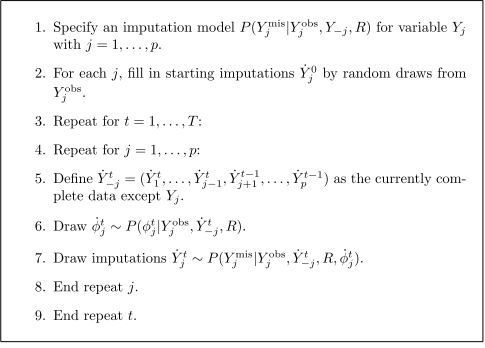
\includegraphics[width=0.6\textwidth]{fcs_algo}
  \caption{FCS imputation pseudocode, taken from \cite{VanBuuren2012}}
\label{fig:fcsexample}
\end{figure}
 \note{ Observe how the previous imputation Y_j^(t-1) only enters the current imputation
 through its relation with other variables, and not directly. This makes convergence very fast
}
\end{frame}

%moved this to intro 666
\begin{frame}{FCS Pros and Cons}
Pros
 \begin{itemize}
  \item Flexible
  \item Easy to specify models
  \item Handles mixed continuous categorical data
  \item Yeilds unbiased estimates with appropriate coverage
 \end{itemize}

 Cons
 \begin{itemize}
  \item No guarantee that full conditionals are compatible
  \item Takes time to set up
  \item Gets much harder as sample size increases to specify models
 \end{itemize}

\end{frame}

\subsection{Application}
\begin{frame}{Imputation with the Cancer Data}

 \begin{itemize}
  \item MAR assumption seems reasonable
  %\item FCS over JM due to nature of data
  \item $m=50$ datasets
  \item 40 iterations
  %\item Check for convergence and validity
 \end{itemize}

\end{frame}

%issues were here


\begin{frame}{Convergence}
 
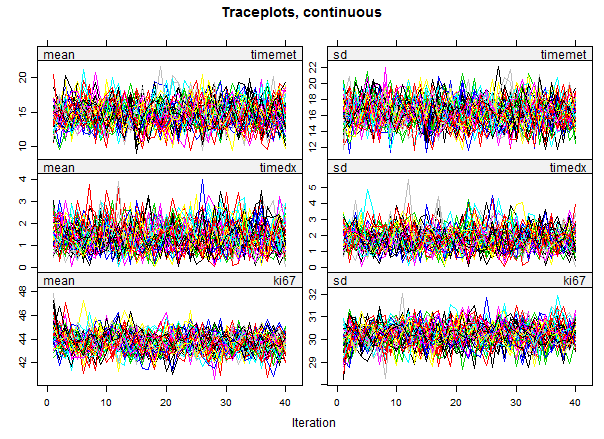
\includegraphics[width=.5\textwidth]{traceplots1}%
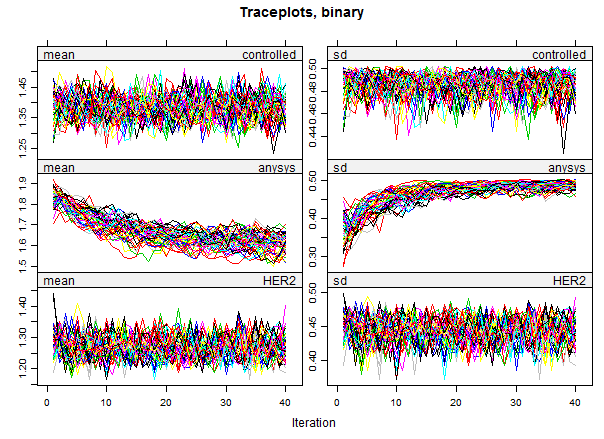
\includegraphics[width=.5\textwidth]{traceplots2} 

\note{On convergence, the different streams should be freely intermingled with one another,
without showing any definite trends. Convergence is diagnosed when the variance between different 
sequences is no larger than the variance within each individual sequence.
We do mean, because without it, we would have 50*missing num for each
var, and it would be very hard to read}

\end{frame}

\begin{frame}{Validity Checks}
%might want to pick better ones
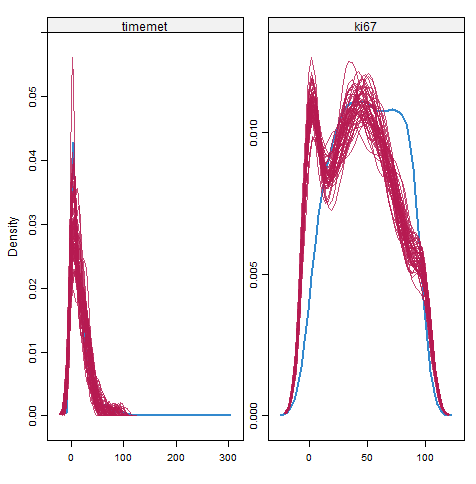
\includegraphics[width=.5\textwidth]{cont_densplot}%
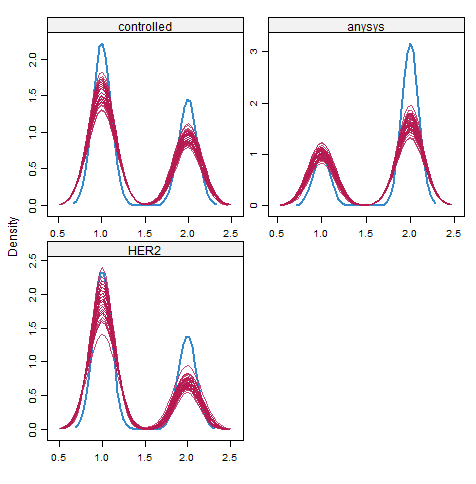
\includegraphics[width=.5\textwidth]{discrete_densplot} 
\end{frame}

\begin{frame}{MI data Breakdown}
\begin{table}[!ht]
\adjustbox{max height=\dimexpr\textheight-5.5cm\relax,
           max width=\textwidth}{
\centering
\begin{tabular}{|r|c|c|c|c|}
\hline
\multicolumn{1}{|l|}{}                            & \begin{tabular}[c]{@{}c@{}}Sys therapy \\ available case\end{tabular} & \begin{tabular}[c]{@{}c@{}}Sys therapy \\ MI\end{tabular} & \begin{tabular}[c]{@{}c@{}}No Sys therapy \\ available case\end{tabular} & \begin{tabular}[c]{@{}c@{}}No Sys therapy \\ MI\end{tabular} \\ \hline
\multicolumn{1}{|l|}{Age (mean,sd)}               & 51.4(10.8)                                                            & 51.2(10.9)                                                & 52.7(11.9)                                                               & 52.9(11.4)                                                   \\ \hline
\multicolumn{1}{|l|}{Breast Cancer subtype}       &                                                                       &                                                           &                                                                          &                                                              \\ \hline
HR+/HER2-                                         & 27\%                                                                  & 31\%                                                      & 28\%                                                                     & 33\%                                                         \\ \hline
HR+/HER2+                                         & 19\%                                                                  & 18\%                                                      & 12\%                                                                     & 13\%                                                         \\ \hline
HR-/HER2+                                         & 22\%                                                                  & 20\%                                                      & 15\%                                                                     & 12\%                                                         \\ \hline
Triple negative                                   & 32\%                                                                  & 32\%                                                      & 45\%                                                                     & 42\%                                                         \\ \hline
\multicolumn{1}{|l|}{Prior therapies for stage 4} & 1(0-3)                                                                & 2(0-4)                                                    & 2(0-4)                                                                   & 2(0-4)                                                       \\ \hline
\multicolumn{1}{|l|}{Single brain lesion}         & 25\%                                                                  & 23\%                                                      & 23\%                                                                     & 20\%                                                         \\ \hline
\multicolumn{1}{|l|}{Controlled extra-cranial}    & 40\%                                                                  & 40\%                                                      & 35\%                                                                     & 36\%                                                         \\ \hline
\multicolumn{1}{|l|}{ECOG 0-1}                    & 84\%                                                                  & 70\%                                                      & 53\%                                                                     & 40\%                                                         \\ \hline
\multicolumn{1}{|l|}{Local Therapy}               &                                                                       &                                                           &                                                                          &                                                              \\ \hline
Resection Alone                                   & 5\%                                                                   & 5\%                                                       & 9\%                                                                      & 7\%                                                          \\ \hline
SBRT alone                                        & 13\%                                                                  & 12\%                                                      & 9\%                                                                      & 8\%                                                          \\ \hline
WBRT                                              & 60\%                                                                  & 59\%                                                      & 52\%                                                                     & 53\%                                                         \\ \hline
Resection/SBRT+WBRT                               & 12\%                                                                  & 14\%                                                      & 10\%                                                                     & 8\%                                                          \\ \hline
no local therapy                                  & 10\%                                                                  & 10\%                                                      & 20\%                                                                     & 23\%                                                         \\ \hline
\end{tabular}
}
\caption{Characteristics of available case data versus MI data}
\label{table:chartab}
\end{table}
 
\end{frame}

\subsection{Rubin's Rules}
\begin{frame}{Rubin's Rules}
 Let
 \begin{itemize}
  \item $\hat{Q}_i$ be the scientific estimand from the $i^{th}$ MI dataset
  \item $U_i$ be the variance-covariance matrix of the $i^{th}$ MI estimand
 \end{itemize}
Then
\begin{itemize}
 \item The MI estimate is given by
 $\bar{Q}=\frac{1}{m}\sum_{i=1}^{m}\hat{Q}_i$
 \item The MI ``within'' variance is given by
 $\bar{U}=\frac{1}{m}\sum_{i=1}^{m}U_i$
 \item the MI ``between'' variance is given by
 $B=\frac{1}{m-1}\sum_{i=1}^{m}(\hat{Q}_i - \bar{Q})(\hat{Q}_i - \bar{Q})'$ % matrix notation?
   \item Total variance given by \cite{Rubin1987}
  $$T=\bar{U}+B +\frac{B}{m}$$
\end{itemize}

\end{frame}

%I'm not sure where I want this to be 666
\begin{frame}{Inference with Rubin's Rules}
 \begin{itemize}
  \item Assume that with complete data, inference on the estimand
  Q would be based on the statement $(Q- \hat{Q})\sim N(0,U)$
  \begin{itemize}
   \item $\hat{Q}$ is the statistic estimating Q
   \item $U$ is the variance-covariance of $(Q-\hat{Q})$
  \end{itemize}
   \item Since true T is not known, then
  $$\frac{Q-\hat{Q}}{\sqrt{T}}\sim t_{\nu}$$
  \item $\nu$ is given by \cite{Barnard1999}
  $$\nu=\frac{\nu_{old}\nu_{obs}}{\nu_{old}+\nu_{obs}}$$
\item Where $\nu_{obs}=\frac{\nu_{com}+1}{\nu_{com}+3}\nu_{com}(1-\frac{B + B/m}{T})$
\item $\nu_{com}$ is the hypothetical complete sample degrees of freedom
\item $\nu_{old}=\frac{m-1}{(\frac{B + B/m}{T})^2}$ 
 \end{itemize}

 \note{Requires normality
if not normal, transform}
\end{frame}